\documentclass[4paper]{article}
\usepackage[spanish]{babel}
%\usepackage[ansinew]{inputenc}
\usepackage[utf8x]{inputenc}
%\usepackage[utf-8]{inputenc}
%\usepackage[T1]{fontenc}
\usepackage{graphicx}
\usepackage{multicol}
\usepackage{float}
%\usepackage{longtable}
%\usepackage{array}
%\usepackage{multirow}
%\usepackage[latin1]{inputenc}
%\inputencoding{latin}
\usepackage{hyperref}
\newcommand{\J}{JavaScript}
\newcommand{\N}{node.js}

%\newcommand{\j}{JavaScript }
%%%%%%%%%%%%%%%%%%%%%%%%%%%%%%%%%%%%%
%Para escribir codigo en latex
\usepackage{listings}
\usepackage{color}


\definecolor{lightgray}{rgb}{.9,.9,.9}
\definecolor{darkgray}{rgb}{.4,.4,.4}
\definecolor{purple}{rgb}{0.65, 0.12, 0.82}

\lstdefinelanguage{JavaScript}{
  keywords={typeof, new, true, false, catch, function, return, null, catch, switch, var, if, in, while, do, else, case, break},
  keywordstyle=\color{blue}\bfseries,
  ndkeywords={class, export, boolean, throw, implements, import, this},
  ndkeywordstyle=\color{darkgray}\bfseries,
  identifierstyle=\color{black},
  sensitive=false,
  comment=[l]{//},
  morecomment=[s]{/*}{*/},
  commentstyle=\color{purple}\ttfamily,
  stringstyle=\color{red}\ttfamily,
  morestring=[b]',
  morestring=[b]"
}

\lstset{
   language=JavaScript,
   backgroundcolor=\color{lightgray},
   extendedchars=true,
   basicstyle=\footnotesize\ttfamily,
   showstringspaces=false,
   showspaces=false,
  % numbers=left,
   numberstyle=\footnotesize,
   numbersep=9pt,
   tabsize=2,
   breaklines=true,
   showtabs=false,
   captionpos=b
}
%%%%%%%%%%%%%%%%%%%%%%%%%%%%%%%%%%%%%%%%
\renewcommand{\tablename}{Tabla}
\renewcommand{\S}{Introducción a \N}
\author{Manuel Molino Milla}
\title{\textbf{\S}}
\date{\today}

\begin{document}
\maketitle 
\tableofcontents
\newpage

\section{Introducción}
\subsection{Ejemplo servidor web en node}
\begin{lstlisting}
const http = require('http')
const hostname = '127.0.0.1'
const port = 3000
const server = http.createServer((req, res) => {
    res.statusCode = 200
    res.setHeader('Content-Type', 'text/plain')
    res.end('Hello World\n')
})
server.listen(port, hostname, () => {
console.log(`Server running at http://${hostname}:${port}/`)
})
\end{lstlisting}
\subsection{¿Qué es \N}
\begin{itemize}
\item Es una plataforma en el lado del servidor.
\item Se basa en el motor \emph{V8 de google}. Aprovechando el motor V8 permite a \N ~ proporcionar un entorno de ejecución del lado del servidor que compila y ejecuta javascript a velocidades increíbles.
\item Fue desarrollado por Ryan Dahl en 2009.
\item Se basa en eventos y sobre todo es no bloqueante.
\item Es \emph{open source} y corre en todos los sistemas operativos.
\item Encontramos proyectos de \N ~ en compañias como \emph{eBay, General Electric, GoDaddy, Microsoft, PayPal, Uber, \dots}
\item Ofrece muy buena gestión de paquetes (librerías) gracias a \emph{npm}
\end{itemize}
\subsection{¿Por qué javascript del lado del servidor?}
\begin{itemize}
\item Encontramos \J ~ en gran número de páginas web y cada vez más código.
\item Generalmente la parte del servidor quedaba relegada a otras soluciones como \emph{php+apache} o \emph{servlets de java} o \emph{microsoft IIS+.NET o C\#}
\item \J ~  tiene la ventaja de poseer un excelente modelo de eventos, ideal para la programación asíncrona.
\item \J ~ es conocido por muchos programadores.
\end{itemize}
%\subsection{¿Qué problema resuelve Node?}
%\begin{itemize}
%\item En lenguajes como Java y PHP, cada conexión genera un nuevo hilo que potencialmente viene acompañado de 2 MB de memoria.
%\item  En un sistema que tiene 8 GB de RAM, esto da un número máximo teórico de conexiones concurrentes de cerca de 4.000 usuarios.
%\item A medida que crece el  número de usuarios se necesitará agregar más servidores.
%\item Por todas estas razones, el cuello de botella en toda la arquitectura de aplicación Web (incluyendo el rendimiento del tráfico, la velocidad de procesador y la velocidad de memoria) era el número máximo de conexiones concurrentes que podía manejar un servidor.
%\item Node resuelve este problema cambiando la forma en que se realiza una conexión con el servidor.
%\end{itemize}
%\subsection{Procesos bloqueantes}
%\begin{itemize}
%\item \N ~ se caracteriza porque es \textbf{no bloqueante} y \textbf{orientado a eventos}
%\item Es similar como un navegador maneja \J.
%\item Fijándonos en los siguientes datos:
%\end{itemize}
%\begin{center}
%\begin{tabular}{|c|c|}
%\hline
%L1 cache read  & 0.5 nanoseconds  \\
%\hline
%L2 cache read & 7 nanoseconds\\
%\hline
%RAM & 100 nanoseconds\\
%\hline
%Read 4 KB randomly from SSD & 150,000 ns\\
%\hline
%Read 1 MB sequentially from SSD & 1,000,000 ns\\
%\hline
%Read 1 MB sequentially from disk & 20,000,000 ns\\
%\hline
%\end{tabular}
\begin{itemize}
\item Observamos que estas operaciones I/O son bastante costosas y cuando se ejecutan dentro de un programa, este deberá esperar a que termine dicha operación para seguir la ejecución normal del programa.
\end{itemize}
\newpage

Ejemplo de programa:
\begin{lstlisting}
let fs = require('fs');
console.log('1');
let archivo = fs.readFileSync('./datos.csv', 'utf-8');

console.log(archivo);
console.log('2');

\end{lstlisting}

\begin{itemize}
\item La función \emph{readFileSync} se encarga de llamar al SO para proceder a la lectura de un fichero de texto.
\item Esto es un cuello de botella, hasta que no se acabe la lectura no podremos continuar el programa.
\item Se trata de una operación bloqueante, hasta que no acabe no prosigue el programa.
\item Este modelo es costoso y presenta mucha latencia, pues cada proceso tiene asociado una memoria y un estado que no se libera hasta que el programa no acabe.
\item Una forma de solucionar esto es usando \emph{hilos}, este es un ejemplo en \emph{Java}:
\end{itemize}

\begin{lstlisting}
public class TestHilos {
  public static void main(String[] args) {
  // lanzamos hilo independiente que se para 5 segundos
  // simula un proceso costoso I/O
    System.out.println("Antes de llamar al hilo");
    Thread lanzarHilo = new Thread(new HiloIndependiente());
    lanzarHilo.start();
    System.out.println("Despues del hilo");
    // paramos el programa principal 5 segundos
    // simula un proceso costoso I/O
    System.out.println("Sin hilos, comienzo");
    try {
      Thread.currentThread().sleep(5_000); 
    } catch (InterruptedException e) {
      e.printStackTrace();
    }
    System.out.println("Sin hilos, fin");
  }
}
class HiloIndependiente implements Runnable{
  @Override
  public void run() {
    try {
      Thread.currentThread().sleep(5_000);
    } catch (InterruptedException e) {
    // TODO Auto-generated catch block
      e.printStackTrace();
    }
  }
}
\end{lstlisting}

\begin{itemize}
\item El uso de hilos hace que puedan compartirse datos en el mismo espacio de memoria donde se ejecuta el proceso.
\item El problema que surge es el de compartición de recursos. Debemos sincronizar los mismos, esto dificulta la programación.
\item En el caso de los navegadores, la gestión I/O es diferente.
\item Ocurren fuera del \emph{hilo principal} y un \emph{evento} es emitido cuando I/O finaliza.
\item El evento es manejado por una \emph{callback} 
\item Este tipo de gestión I/O es \emph{no bloqueante} y \emph{asíncrona}
\item Como I/O es no va a bloquear, el hilo principal continua y getiona otros eventos sin esperar a la culminación del proceso I/O
\item \N ~ trabaja de forma similar.
\end{itemize}


\begin{figure}[H]
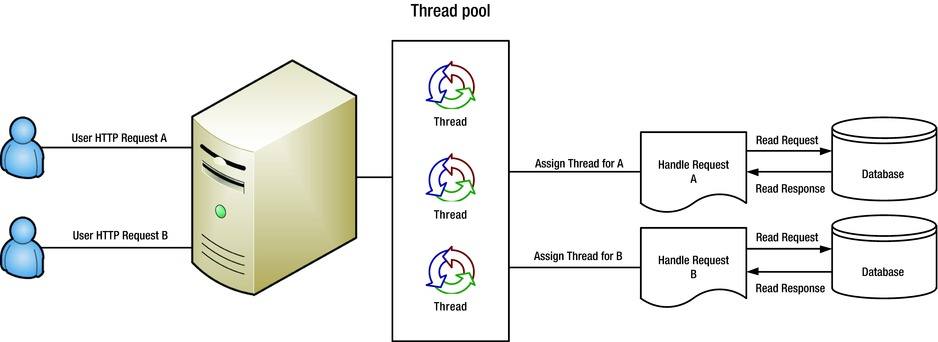
\includegraphics[scale=1]{../imagenes/server.jpg}
\caption{Servidor tradicional}
\end{figure}

\begin{figure}[H]
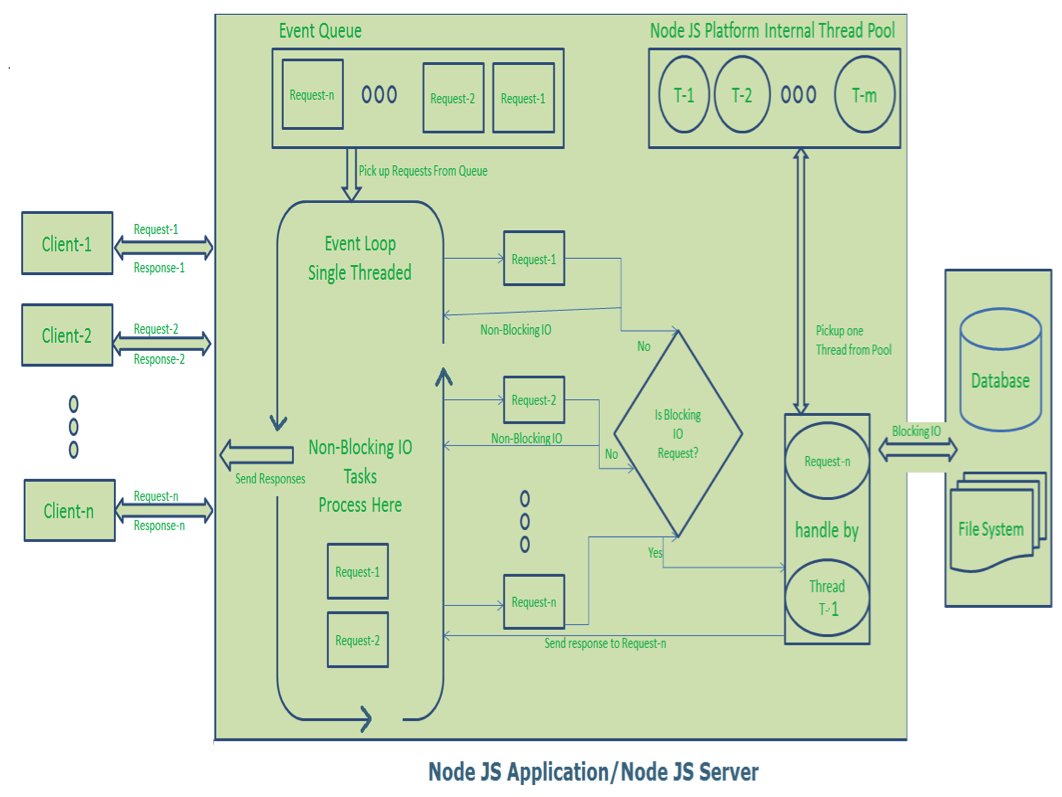
\includegraphics[scale=0.3]{../imagenes/eventloop.png}
\caption{Servidor no bloqueante}
\end{figure}

\begin{figure}[H]
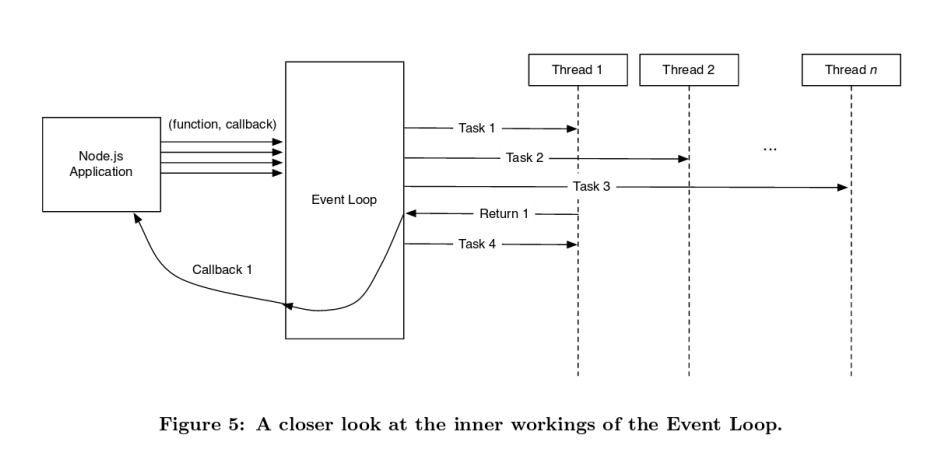
\includegraphics[scale=0.5]{../imagenes/hilos.png}
\caption{node js}
\end{figure}

\newpage
\subsection{callback}

\begin{itemize}
\item Es una función que hace que \N ~ trabaje de forma \emph{asíncrona}
\item El caso de la lectura del fichero
\end{itemize}
En el caso \emph{síncrono}:
\begin{lstlisting}
const fs = require('fs')

const data = fs.readFileSync('/etc/passwd', 'utf8')
console.log(data)

console.log('Fin del programa');

\end{lstlisting}

Y el caso \emph{asíncrono}:
\begin{lstlisting}
const fs = require('fs')

const data = fs.readFile('/etc/passwd','utf8', (err,data) => {
  if (err)
   throw err
  else
   console.log(data) // => muestra el contenido del fichero
})

console.log('fin del programa')
\end{lstlisting}
Usando promesas:
\begin{lstlisting}
const fs = require('fs')

fs.readFileAsync = filename => {
    return new Promise((resolve, reject) => {
        fs.readFile(filename, 'utf8',  (err, data) => {
            if (err) reject(err)
            resolve(data)
        });
    });
};


const getFile = file =>  fs.readFileAsync(file)


getFile('/etc/passwd').then(
        data => console.log(data)
).catch(
        err => console.log(err)
)

\end{lstlisting}

\newpage
Otro ejemplo sería un programa que con la ayuda de una función tarda medio segundo en calcular el valor de la suma, simulando un proceso bloqueante. Nos ayudamos de la función \emph{setTimeout} cuyo segundo argumento es el tiempo de respuesta:
En el caso síncrono el código sería:
\begin{lstlisting}
const suma = (numero_uno,numero_dos) => {
   setTimeout( () => {
      return numero_uno + numero_dos
   }, 500)
}

const resultado = suma(2,5)
console.log(resultado);  //undefined
\end{lstlisting}
Y en el caso asíncrono sería:
\begin{lstlisting}
const suma = (numero_uno,numero_dos,callback) => {
   setTimeout( () => {
      callback(numero_uno + numero_dos)
   }, 500)
}
suma(2 ,5 , resultado => {
   console.log(resultado)
})

\end{lstlisting}
\begin{itemize}
\item El parámetro \emph{callback}. Éste nos ayudará a retornar el resultado cuando esté listo.
\item El valor devuelto por la función no se asigna a una variable, sino se usa como parámetro la función que devuelve el valor.
\end{itemize}
Conclusiones:
\begin{itemize}
\item Las callback en vez de retornar el resultado como la mayoría de las funciones, estás toman cierto tiempo en devolver el resultado.
\end{itemize}

Usando promise:
\begin{lstlisting}
const suma = (numero_uno,numero_dos) => {
    return new Promise((resolve, reject) => {
        setTimeout( () => {
             if (!numero_uno && !numero_dos)
                  reject(new Error('faltan numeros'))
             resolve(numero_uno + numero_dos)
        },500)
    })
}

suma(2,5).then(console.log)
suma().catch(console.log)
\end{lstlisting}

\newpage

Usando async awayt
\begin{lstlisting}
const suma = (numero_uno,numero_dos) => {
        return new Promise((resolve, reject) => {
                setTimeout( () => {
                        if (!numero_uno && !numero_dos)
                                reject(new Error('faltan numeros'))
                        resolve(numero_uno + numero_dos)
                },2500)
        })
}

const resultado1 = async () =>  console.log(await suma(2,5))
resultado1()
const resultado2 = async () =>  console.log(await suma())
resultado2()
\end{lstlisting}

Hay que tener cuidado en el caso que usemos funciones predefinidas que no sean asíncronas, como puede ser la función \emph{sort} que ordena un array. Para esto usamos \emph{process.nextTick}
\begin{lstlisting}
function coleccion (valor) {
  var _valor = valor;
  var funcionDeComparacion = function (elem1, elem2) {return elem1 -elem2;};
  return {
    ordenar : function(callback) {
      process.nextTick(function() {
        callback(_valor.sort(funcionDeComparacion));
      });
    }
  }
}
\end{lstlisting}

\newpage
\subsection{Programación orientada a eventos en \N}
\begin{itemize}
\item \N ~ funciona en un único hilo de ejecución, pero soporta concurrencia mendiante eventos y callback.
\item Los eventos son parecidos a las callback, pero NO lo son.
\item Las callback retornan un resultado cuando una función asíncrona las usa.
\item En cambio existen funciones que escuchan eventos y actúan como observadoras.
\end{itemize}

Ejemplo de un servidor web usando eventos:
\begin{lstlisting}
var http = require("http");
var server = http.createServer();

server.on("request", function (req, res) {
  res.statusCode = 200;
  res.setHeader('Content-Type', 'text/plain');
  res.end('Hello World\n');
});

server.listen(3000);
\end{lstlisting}
Y usando callback (Sacado de la página oficial)
\begin{lstlisting}
const http = require('http');

const hostname = '127.0.0.1';
const port = 3000;

const server = http.createServer((req, res) => {
  res.statusCode = 200;
  res.setHeader('Content-Type', 'text/plain');
  res.end('Hello World\n');
});

server.listen(port, hostname, () => {
  console.log(`Server running at http://${hostname}:${port}/`);
});
\end{lstlisting}
El mismo servidor, también usando callback, pero de diferente forma:
\begin{lstlisting}
var http = require("http").createServer(function(req, res) {
  res.statusCode = 200;
  res.setHeader('Content-Type', 'text/plain');
  res.end('Hello World\n');
}).listen(3000);
console.log("Server is listening");
\end{lstlisting}

\newpage

\subsection{Módulos en \N}
\begin{itemize}
\item Es importante la organización del código, sobre todo cuando el número de líneas aumenta.
\item Para esto podemos crear módulos independientes.
\item Usamos la palabra reservada \emph{exports}
\end{itemize}
Ejemplo 1, fichero \emph{geometria.js}:
\begin{lstlisting}
exports.area = function (r) {
  return 3.14 * r * r;
};
exports.circumference = function (r) {
  return 3.14 * 3.14 * r;
};
\end{lstlisting}
Qué lo podemos usar:
\begin{lstlisting}
var geo = require('./geometria.js');
console.log(geo.area(2));
\end{lstlisting}
Otra forma de trabajar es usar \emph{modules.exports} y clousures
\begin{lstlisting}
function circunferencia (radio) {
  _radio = radio;
  return {
    area:      function() { return _radio * _radio * 3.14 ; },
    perimetro: function() { return 2 * 3.14 * _radio }
  }
}
module.exports = circunferencia;
#module.exports.circunferencia = circunferencia (de otra manera)
\end{lstlisting}
Y crear un main.js como:
\begin{lstlisting}
var circunferencia = require('./circunferencia');

console.log(circunferencia(4).area());
console.log(circunferencia(4).perimetro());
\end{lstlisting}
\newpage
Y usando un constructor quedaría:
\begin{lstlisting}
function Circunferencia (radio) {
  this.radio = radio;
}

Circunferencia.prototype = {
  area     : function() { return this.radio * this.radio * 3.14; },
  perimetro: function() { return this.radio * 2 * 3.14; }
}

module.exports = Circunferencia;
\end{lstlisting}
Y el main.js:
\begin{lstlisting}
var Circunferencia = require('./Circunferencia');

var circunferencia = new Circunferencia(4);

console.log(circunferencia.area());
console.log(circunferencia.perimetro());
\end{lstlisting} 
Otro ejemplo puede ser la configuración del acceso a una BD:
\begin{lstlisting}
var db_config = {
  server: "0.0.0.0",
  port: "3306",
  user: "mysql",
  password: "mysql"
};
module.exports = db_config;
\end{lstlisting}
Y su uso podría ser:
\begin{lstlisting}
var config = require('./config.js');
console.log(config.user);
\end{lstlisting}


\newpage

%\subsection{Ejercicios}
%\begin{itemize}
%\item Crea un módulo denominado \emph{estadistica.js} que dado una colección de números nos diga:
%\begin{itemize}
%\item El número de números de la colección.
%\item El valor mas alto.
%\item El valor mas bajo.
%\item Dado un número como argumento, nos indique cuantas veces se repite en la colección.
%\item No entregue la colección ordenada.
%\item El valor promedio de la colección.
%\end{itemize}
%\item Convierte el ejercicio de \emph{cadenas.js} en un módulo.
%\item Idem con el ejercicio de dni y nif.
%\end{itemize}

\subsection{npm}
\begin{itemize}
\item Es el gestor de módulos de \N
\item Viene integrado en el proceso de instalación de \N
\item Es la herramienta perfecta y necesaria en cuando a manejo de dependencias se refiere.
\end{itemize}
Los comandos mas interesantes son:
\begin{description}
\item[npm init] permite crear, modificar y generar un \emph{package.json}
\item[npm search \emph{nombre-del-modulo} o \emph{palabra-clave}]  permite buscar en el registro de npm, algun modulo acerca de la palabra clave
\item[npm info nombre-del-modulo] Muestra información en formato json acerca de nombre-del-modulo
\item[npm ls, npm la, npm ll, npm list] lista los paquetes actualmente instalados en un determinado directorio. En formato de tree.
\item[npm outdated] busca si hay versiones más nuevas acerca de los modulos instalados en el directorio actual.
\item[npm install \emph{nombre-del-módulo}] instala el módulo en el directoria actual en una carpeta denominada \emph{modules}. Si se hace con la opción \emph{-g} se instala de forma global en el sistema. Y con la opción \emph{--save} se añade como dependencia al fichero \emph{package.json}
\item[npm uninstall \emph{nombre-del-módulo}] desinstala el módulo determinado. Admite las opciones anteriores de la instalación.
 \end{description}
 
 \newpage
\subsubsection{package.json}
Se genera con el comando \emph{npm init}
Ejemplo
\begin{lstlisting}
> npm init --yes
  Wrote to /home/ag_dubs/my_package/package.json:

  {
    "name": "my_package",
    "description": "",
    "version": "1.0.0",
    "main": "index.js",
    "scripts": {
      "test": "echo \"Error: no test specified\" && exit 1"
      "star": "npm run index.js"
    },
    "repository": {
      "type": "git",
      "url": "https://github.com/ashleygwilliams/my_package.git"
    },
    "keywords": [],
    "author": "",
    "license": "ISC",
    "bugs": {
      "url": "https://github.com/ashleygwilliams/my_package/issues"
    },
    "homepage": "https://github.com/ashleygwilliams/my_package"
  }
\end{lstlisting}
Existe un fichero \emph{package-lock.json} que se genera automáticamente a partir de la versión 5. La finalidad es que se pueda mantener un detalle específico de las versiones de dependencias que tenés instaladas en el proyecto. Esto sirve, por ejemplo, para garantizar que todos los que trabajando en un proyecto tenga instaladas las mismas versiones de paquetes y evitar tener problemas con distintas versiones de dependencias.\\
En el caso de las dependencias debemos tener en cuenta:
\begin{lstlisting}
Si escribimos ~0.13.0 significa que queremos solo actualizar a partir de esa version, ejemplo 0.13.1. Pero no podemos superar la 0.13, 0.14.0 no seria posible
Si escribimos ^0.13.0 si seria posible
\end{lstlisting}
\subsection{Leyendo de la entrada estándar}
\begin{lstlisting}
const readline = require('readline').createInterface({
   input: process.stdin,
   output: process.stdout
})
readline.question(`What's your name?`, (name) => {
   console.log(`Hi ${name}!`)
   readline.close()
})
\end{lstlisting}

\subsection{Ejercicio final}

Usando la base de datos del tema anterior, realiza un programa que nos crea un menú simple que solicite la operación a realizar sobre la BD (CRUD), pudiendo solicitar por consola datos para realizar consultas, insercciones, etc. El programa debe -por ejemplo- realizar la siguientes acciones:
\begin{enumerate}
\item Listar todos los datos  que se encuetran en la BD
\item Listar todos las ciudades, dado un país
\item Insercción de un nuevo documento.
\item Borrado por nombre de ciudad
\item Actualización de latitud y longitud de una ciudad
\end{enumerate}

Usa la siguiente documentacion:\\
\begin{center}
\href{https://mongodb.github.io/node-mongodb-native/}{Conectar mongo con node}\\
\href{https://teamtreehouse.com/community/how-to-get-input-in-the-console-in-nodejs}{Lectura desde consola con node}\\
\href{https://www.npmjs.com/package/simple-menu}{Simple menu en node}
\end{center}
%Tenemos el fichero \emph{datos.csv} que contempla 1000 registros de datos con el nombre, primer apellido, email, edad y sexo, y queremos implementar un programa en \emph{nodejs} que primero lea dicho fichero como argumento del programa, ejemplo:
%\begin{quote}
%node leerFicheroCSV.js datos.csv
%\end{quote}
%Nos de un mensaje en el caso que no encuetre el fichero y la lectura no debe ser bloqueante, comprueba dicho requisito\\
%A la vez que se leen los datos, se crea un array de objetos persona que tienen como atributos cada uno de los campos del fichero CSV.\\
%En un módulo aparte, crea un programa que dada la colección de objetos anterior nos de:
%\begin{itemize}
%\item La mayor edad y menor edad como un objeto.
%\item Una colección de objetos de persona con mas edad.
%\item Dado el sexo (M o F) nos de una lista de personas de igual sexo.
%\end{itemize} 
\end{document}
